\documentclass{zarticle}
\usepackage{tikz}
\usetikzlibrary{shapes.symbols,shapes.geometric,decorations.pathreplacing,calc}
\addbibresource{shared.bib}
\definecolor{todocolor}{RGB}{127,0,0}
\def\todo#1{{\color{todocolor}\bfseries [#1]}}
\def\needcite#1{\todo{cite: #1}}
\begin{document}

\title{Unmasking Web Users and Activities:
  A review of the literature on traffic analysis of the modern Internet}
\author{Zachary Weinberg}
\date{\today}
\maketitle

\begin{abstract}
Abstract abstract, abstract abstract abstract.
\end{abstract}

\section{Introduction}

\emph{Traffic analysis} is the craft of deducing information about the
content of an encrypted message from any data that remains observable
despite the encryption, such as its sender, recipient, length, time of
transmission, or its relationship to other events.  Classically, one
might deduce that a naval vessel has received new orders if it
abruptly changes course shortly after an encrypted radio broadcast.
\todo{More history?}

A protocol which provides cryptographic confidentiality, integrity,
and authenticity on top of a best-effort, cleartext infrastructure is
generally referred to as a “secure channel,” but traffic analysis can
extract information from most secure-channel protocols used on the
modern Internet, damaging to some extent the theoretical guarantee of
confidentiality.  In this paper we will review the state of the art in
traffic analysis specifically of HTTP (World Wide Web) transactions
relayed through proxies which are intended to guarantee the anonymity
of their users.

\subsection{Levels of Anonymity}

“Anonymity” is an overloaded term.  Following
Pfitzmann~\cite{pfitzmann2010terminology}, in this paper we will
distinguish three levels of anonymity protection.  An \emph{overt}
secure protocol (such as TLS or SSH) conceals the content of each
message but makes no effort to hide the sender and recipient of each
message (that is, the IP source and destination addresses).  The
information that Alice did at some point talk to Bob has sometimes
been enough to send Alice to prison!\footnote{As an extreme example,
  the Soviet Union notoriously criminalized “contacts leading to
  suspicion of espionage.”~\cite{solzh1974gulag:svpsh}} An
eavesdropper can also learn the amount of application data each packet
carries, its position within a TCP stream, and other metainformation,
such as any TCP options that are present.

An \emph{unlinkable} protocol additionally prevents an eavesdropper at
any single point in the network from learning both the sender and the
recipient of each message.  Depending on the eavesdropper's location,
they may be able to learn that Alice is sending messages to
\emph{someone}, or that Bob is receiving messages from \emph{someone},
but they should not be able to learn that Alice is communicating with
Bob.  Unlinkability is the level of protection provided by most
anonymity services in wide use on the public Internet.  It is normally
achieved by passing the traffic through one or more relays, such that
each knows only the previous and next hop; a secure channel is still
established end-to-end, so the relays themselves cannot observe
message contents.  This design originates with \textcite{chaum1981mix}
and will be discussed in more detail below.

Finally, \emph{unobservable} traffic is (computationally)
indistinguishable from background chatter, so an eavesdropper cannot tell
whether any given station is talking to \emph{anyone}.
Unobservability represents an ideal; although there are a few
proposals, no unobservable protocol has been made practical.
\todo{expand}

\subsection{Attacking Unlinkability}

There are a wide variety of threat models in the literature for
traffic-analytic attackers on unlinkable channels.  The attacker may
be located at several different places within the network, and may
have one, two, or several listening posts.  It may be strictly an
eavesdropper, or may be allowed to generate its own traffic, or may
even operate its own malicious relays.  It may be able to communicate
overtly with its victims, for instance by enticing them to visit an
attacker-controlled website; this is more powerful than it might
sound, since a malicious website can execute code (in a restricted,
but not at all foolproof, environment) on its victims'
computers.~\cite{barth2008securing} However, “Byzantine” attacks, in
which the attacker interferes with the correct operation of the
unlinkable channel protocol, are considered a separate class of
threat.  The attacker's goals are even more diverse, ranging from
the deduction of encrypted channel content to tracing messages through
the relay chain to identifying communicants. \todo{sprinkle cites in
  this paragraph}

Unlinkable protocols don't generally conceal the size or the timing of
messages.  There are exceptions: \citeauthor{chaum1981mix}'s original
design~\cite{chaum1981mix} (intended for email) did include
substantial delays at each relay in order to conceal timing, but this
is not considered acceptable for modern interactive protocols such as
HTTP: current-generation mix networks, such as
Tor~\cite{dingledine2004tor}, treat their \emph{low latency} as a
valuable feature.  Unlinkable channels may or may not conceal the TCP
session to which each packet belongs.  If they don't, this gives the
attacker additional information, particularly for protocols (such as
HTTP) that use many short-lived TCP sessions, as will be discussed
further below.

When an unlinkable protocol uses only one relay, the relay is
colloquially known as a “proxy server,” and is a point of
vulnerability, since it knows the source and destination of every
message.  Even if run with the best of intentions, proxy servers may
come under coercion to expose that information.\footnote{In one
  notorious case from the early Internet, the email relay
  \textsf{anon.penet.fi} shut down under ongoing legal pressure to
  unmask its users.~\cite{newman1996church}} A \emph{mix
  network}~\cite{chaum1981mix} replaces the single relay with a chain
of relays, each of which knows only the previous and next hop;
subverting any one relay thus reveals no more than eavesdropping would
have.  In practice, three relays are used, because a two-relay chain
is insufficient to defend against attacks by pairs of colluding
malicious relays, but a chain of four or more relays offers only
marginal additional security at substantial cost in
latency.~\cite{wright2002analysis,wright2003defending}.

\subsection{Website Fingerprinting}

This review focuses on two classes of traffic analysis attacks, both
of which are referred to in the literature as “website
fingerprinting.”  Both feature an attacker eavesdropping on a
victim-user at or near the victim's location in the network;
specifically, the attacker is assumed to be able to observe traffic
between the victim's computer and the first relay in the unlinkable
channel.  Therefore, the attacker already knows something about the
victim, and their goal is to learn something about what they are using
the unlinkable channel for.  (One result discussed
below~\cite{gong2011remote} suggests the possibility of fingerprinting
from afar by flooding the victim with ICMP “ping” messages, but the
traffic so observed is still the traffic between the victim's computer
and the first relay.)

In one class of fingerprinting attacks, the attacker simply seeks to
determine which Web sites the victim is browsing via the unlinkable
channel; we'll refer to this as the \emph{identify-site} attack.  Some
identify-site attacks we review studied the behavior of proxy servers,
while other papers examined mix networks, and a few compared both.  We
will only highlight which of the two was studied when the difference
matters.

In the other class, the attacker knows or assumes that the victim is
browsing a particular website, and attempts to learn something about
what they're doing there.  This we shall call the \emph{within-site}
attack.  Within-site attacks may be applied to either sort of
unlinkable channel, but unlike identify-site attacks, they are also
relevant to the default \emph{overt} channel used by HTTPS.  They come
in two major subclasses.  \emph{Identify-user} attacks seek to
identify the social network profile belonging to the user doing the
browsing, assuming the adversary doesn't already know this from the
client's IP address.  This can be done, for instance, if users'
profile photos in aggregate are considered public data; \emph{which}
profile photo is linked from a given page is supposed to be secret,
but the photos tend to have unique file sizes, so the adversary can
simply match them against a
database.~\cite{herrmann2012analyzing,pironti2012identifying}
\emph{State-tracing} attacks seek to extract confidential information
from the sequence of observable state transitions in a Web
application.  For instance, reconstructing the sequence of questions
presented by a tax-preparation website may reveal the target's
approximate income, marital status, and other such highly confidential
data.~\cite{zhang2010sidebuster}

\subsection{HTTP's Network Behavior}

The World Wide Web has existed since 1990, and since 1994 it has been
possible to configure individual websites for \emph{overt} secure
communications, using the generic secure-channel protocol known as
TLS.\footnote{TLS stands for \emph{Transport Layer Security}. It is
  also known by the older name SSL, \emph{Secure Sockets Layer};
  technically, newer revisions of the protocol (since 1999) are TLS,
  older are SSL.}  HTTP (\emph{HyperText Transport Protocol}), the
Web's application-layer protocol, has not changed significantly since
the adoption of version 1.1 in 1996.\footnote{In the past few years,
  radical revisions of HTTP, such as Google's SPDY, have been proposed
  and adopted to some extent; we are not aware of any research into
  how this changes the situation for an eavesdropper.}

Whether or not encapsulated in a secure channel, HTTP exhibits
characteristic network behavior which is useful for traffic analysis.
The client always sends first in HTTP, transmitting a \emph{query}
which is met with a \emph{response} from the server.  A TCP connection
can be reused for several query-response pairs, but the client cannot
begin a new query until it has received the complete response to its
previous query, nor can the server begin a response before the query
is fully received.  HTTP 1.1 includes a \emph{pipelining} mechanism
that lifts this restriction, but unlike the rest of protocol 1.1,
pipelining has never seen wide adoption.

Therefore, an eavesdropper at the TCP layer will see each party
alternate between sending and receiving, and the aggregate TCP payload
size of each server-to-client burst is a close approximation to the
file size of the object requested.  To enhance parallelism, browsers
open anywhere between two and ten simultaneous connections to the same
site, allowing them to request several items at once (e.g.\ all the
images referenced by an HTML page); each such connection behaves as
described.

Some, but not all, unlinkable channel protocols disguise the
characteristic HTTP traffic pattern to some extent.  For instance, Tor
multiplexes all proxied TCP connections onto a small number of
long-lived “circuits,” hiding the simultaneous connections aspect of
HTTP.  The alternating send and receive bursts are still visible, but
it is harder to determine the exact size of each item.

\begin{figure*}[t!]%
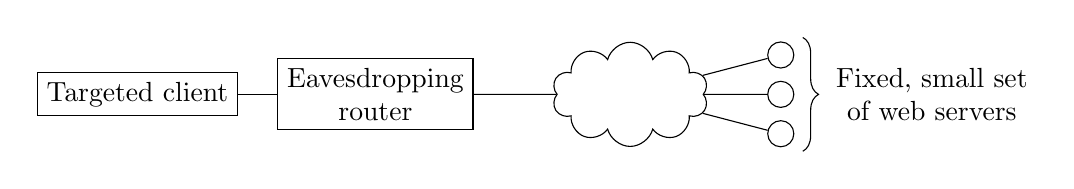
\begin{tikzpicture}[every node/.style={align=center,draw}]
\matrix [draw=none]
{
   \node (a) {Targeted client};
&[5mm]
   \node (b) {Eavesdropping\\router};
&[10mm]
   \node (c) [cloud,aspect=2] {\strut};
&[7.5mm]
   \foreach \y/\l in {5mm/da,0mm/db,-5mm/dc} \node [circle] (\l) at (0,\y) {};
   \coordinate [above=0.5mm] (d0) at (da.north) ;
   \coordinate [below=0.5mm] (d1) at (dc.south) ;
&[1mm]
   \draw [decorate,decoration={brace,amplitude=2mm}] (d0 -| 0,0) -- (d1 -| 0,0);
&[1mm]
   \node (e) [draw=none] {Fixed, small set\\of web servers};
\\
};
\draw (a) edge (b)
      (b) edge (c)
      (c) edge (da)
      (c) edge (db)
      (c) edge (dc)
;
\end{tikzpicture}%
\caption{Laboratory topology for fingerprinting experiments.}%
\label{f:lab.topology}%
\end{figure*}

\begin{figure*}[t!]%
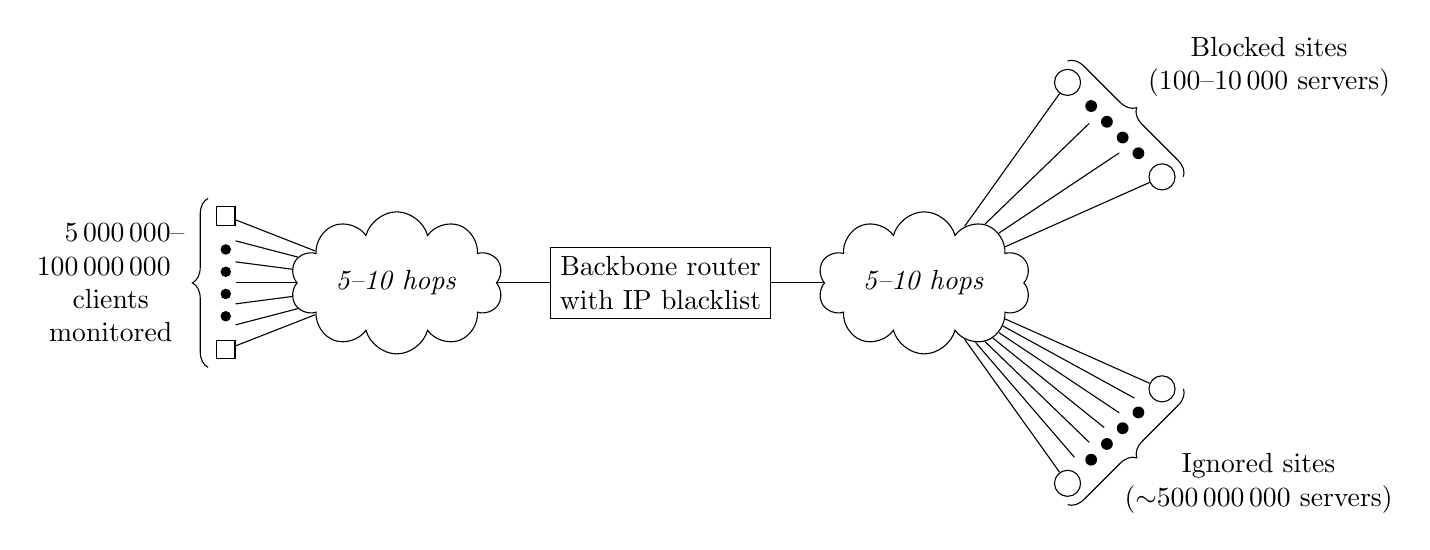
\begin{tikzpicture}[every node/.style={align=center,draw}]
\matrix[draw=none,column sep=3mm,row sep=2mm]
{
&[4mm]
&[3mm]
&[3mm]
&
  \node (t1) [shape=circle] at (-6mm,6mm) {};
  \node (t2) [shape=circle,draw=none] at (-2mm,2mm) {};
  \node (t3) [shape=circle,draw=none] at (2mm,-2mm) {};
  \node (t4) [shape=circle] at (6mm,-6mm) {};
  \foreach \xy in {(-3mm,3mm),(-1mm,1mm),(1mm,-1mm),(3mm,-3mm)}
    \fill \xy circle (0.75mm) ;
\\
\node (c1) at (0,-8.49mm) {};
\node (c2) [draw=none] at (0,-5.66mm) {};
\node (c3) [draw=none] at (0,-2.83mm) {};
\node (c4) [draw=none] at (0,0) {};
\node (c5) [draw=none] at (0,2.83mm) {};
\node (c6) [draw=none] at (0,5.66mm) {};
\node (c7) at (0,8.49mm) {};
  \foreach \xy in {(0,-4.24mm),(0,-1.41mm),(0,1.41mm),(0,4.24mm)}
    \fill \xy circle (0.666mm) ;
&
  \node (cloud1) [cloud,aspect=2] {\textit{5--10 hops}};
&
  \node (eve) {Backbone router\\with IP blacklist};
&
  \node (cloud2) [cloud,aspect=2] {\textit{5--10 hops}};
&
\\
&
&
&
&
  \node (d1) [shape=circle] at (6mm,6mm) {};
  \node (d2) [shape=circle,draw=none] at (4mm,4mm) {};
  \node (d3) [shape=circle,draw=none] at (2mm,2mm) {};
  \node (d4) [shape=circle,draw=none] at (0mm,0mm) {};
  \node (d5) [shape=circle,draw=none] at (-2mm,-2mm) {};
  \node (d6) [shape=circle,draw=none] at (-4mm,-4mm) {};
  \node (d7) [shape=circle] at (-6mm,-6mm) {};
  \foreach \xy in {(-3mm,-3mm),(-1mm,-1mm),(1mm,1mm),(3mm,3mm)}
    \fill \xy circle (0.75mm) ;
\\
};
\draw (cloud1) edge (eve)
      (eve) edge (cloud2) ;
\foreach \n in {c1,c2,c3,c4,c5,c6,c7} \draw (\n) edge (cloud1) ;
\foreach \n in {t1,t2,t3,t4} \draw (cloud2) edge (\n) ;
\foreach \n in {d1,d2,d3,d4,d5,d6,d7} \draw (cloud2) edge (\n);

\draw [decorate,decoration={brace,amplitude=2mm}]
  ($(c1.south west)+(-1mm,-1mm)$) -- ($(c7.north west)+(-1mm,1mm)$) ;
\draw [decorate,decoration={brace,amplitude=2mm}]
  ($(t1.north)+(0,1mm)$) -- ($(t4.east)+(1mm,0)$) ;
\draw [decorate,decoration={brace,amplitude=2mm}]
  ($(d1.east)+(1mm,0)$) -- ($(d7.south)+(0,-1mm)$) ;

\node [draw=none,anchor=east] at ($(c1)!0.5!(c7) + (-4mm,0)$)
 {\phantom{10}5\,000\,000--\\100\,000\,000\phantom{--}\\clients\\monitored}
;
\node [draw=none,anchor=south west] at ($(t1)!0.5!(t4) + (3mm,3mm)$)
 {Blocked sites\\(100--10\,000 servers)}
;
\node [draw=none,anchor=north west] at ($(d1)!0.5!(d7) + (0mm,-1mm)$)
 {Ignored sites\\($\sim$500\,000\,000 servers)}
;
\end{tikzpicture}%
\caption{Model topology for large-scale network censorship.}%
\label{f:cens.topology}%
\end{figure*}

\begin{figure*}[t!]%
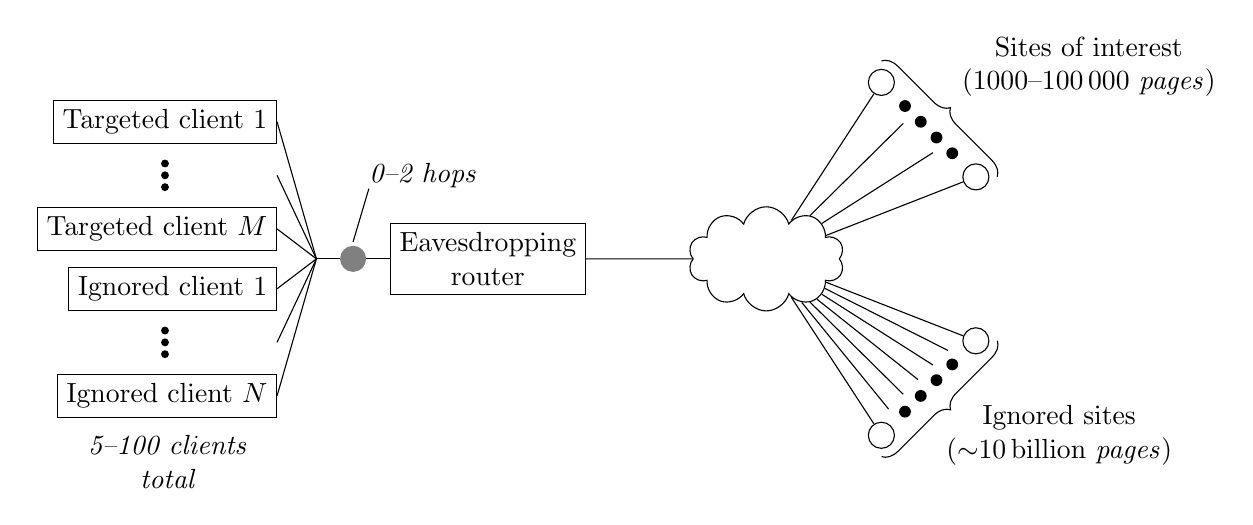
\begin{tikzpicture}[every node/.style={align=center,draw}]
\matrix (a) [draw=none,row sep=2mm,nodes={anchor=east}]
{
  \node (a1) {Targeted client $1$} ;\\
  \foreach \y in {-1.5mm,0,1.5mm}
    \fill (a1.center |- 0,\y) circle (0.5mm) ;\\
  \node (a2) {Targeted client $M$} ;\\
  \node (a3) {Ignored client $1$} ;\\
  \foreach \y in {-1.5mm,0,1.5mm}
    \fill (a1.center |- 0,\y) circle (0.5mm) ;\\
  \node (a4) {Ignored client $N$} ;\\
};
\node [draw=none,below=1mm] at (a4.south) {\itshape 5--100
  clients\\\itshape total} ;
\matrix[draw=none,matrix anchor=b1.west,column sep=3mm,row sep=2mm]
  at ($(a2.east)!0.5!(a3.east) + (5mm,0)$)
{
&
&
&[10mm]
&
  \node (t1) [shape=circle] at (-6mm,6mm) {};
  \node (t2) [shape=circle,draw=none] at (-2mm,2mm) {};
  \node (t3) [shape=circle,draw=none] at (2mm,-2mm) {};
  \node (t4) [shape=circle] at (6mm,-6mm) {};
  \foreach \xy in {(-3mm,3mm),(-1mm,1mm),(1mm,-1mm),(3mm,-3mm)}
    \fill \xy circle (0.75mm) ;
\\
  \coordinate (b1) {};
&
  \node (b2) [draw=none,fill=gray,shape=circle,outer sep=0pt] {};
&
  \node (eve) {Eavesdropping\\router};
&
  \node (cloud) [cloud,aspect=2] {\strut};
&
\\
&
&
&
&
  \node (d1) [shape=circle] at (6mm,6mm) {};
  \node (d2) [shape=circle,draw=none] at (4mm,4mm) {};
  \node (d3) [shape=circle,draw=none] at (2mm,2mm) {};
  \node (d4) [shape=circle,draw=none] at (0mm,0mm) {};
  \node (d5) [shape=circle,draw=none] at (-2mm,-2mm) {};
  \node (d6) [shape=circle,draw=none] at (-4mm,-4mm) {};
  \node (d7) [shape=circle] at (-6mm,-6mm) {};
  \foreach \xy in {(-3mm,-3mm),(-1mm,-1mm),(1mm,1mm),(3mm,3mm)}
    \fill \xy circle (0.75mm) ;
\\
};
\node (b2l) [draw=none,anchor=base west,inner sep=0pt]
  at ($(b2.north)+(2mm,8mm)$) {\textit{0--2 hops}};
\draw (b2l.south west) edge ($(b2.north)+(0,0.5mm)$) ;

\foreach \n in {a1,a2,a3,a4} \draw (\n.east) edge (b1) ;
\draw ($(a1.east)!0.5!(a2.east)$) edge (b1)
      ($(a3.east)!0.5!(a4.east)$) edge (b1) ;

\draw (b1) edge (b2)
      (b2) edge (eve)
      (eve) edge (cloud) ;
\foreach \n in {t1,t2,t3,t4} \draw (cloud) edge (\n) ;
\foreach \n in {d1,d2,d3,d4,d5,d6,d7} \draw (cloud) edge (\n);
\draw [decorate,decoration={brace,amplitude=2mm}]
  ($(t1.north)+(0,1mm)$) -- ($(t4.east)+(1mm,0)$) ;
\draw [decorate,decoration={brace,amplitude=2mm}]
  ($(d1.east)+(1mm,0)$) -- ($(d7.south)+(0,-1mm)$) ;
\node [draw=none,anchor=south west] at ($(t1)!0.5!(t4) + (3mm,3mm)$)
 {Sites of interest\\(1000--100\,000 \emph{pages})}
;
\node [draw=none,anchor=north west] at ($(d1)!0.5!(d7) + (1mm,-1mm)$)
 {Ignored sites\\($\sim$10\,billion \emph{pages})}
;
\end{tikzpicture}%
\caption{Our proposed realistic topology for fingerprinting attacks.}%
\label{f:real.topology}%
\end{figure*}


%% \section{Early Work}

%% The earliest attempts we are aware of, to perform traffic analysis of
%% the Web's protocols, are from 1998 and 2002.
%% \textcite{cheng1998traffic}, the very earliest publicly available
%% analysis, presents a within-site attack on overt HTTPS.  They make use
%% of HTTP's query-response traffic pattern to determine the size of
%% individual pages and/or embedded resources, and then match those sizes
%% against a previously-generated table of sizes for \emph{all} the
%% publicly visible URLs on that site.  They observe that 90\% of HTML
%% files on the sites they studied have unique sizes, and similarly for
%% images (image files almost always have internal compression, so their
%% file size depends on their contents as well as their dimensions).
%% They do not explicitly consider how long an identification might last,
%% but they do mention modeling a dynamically updated page as a
%% collection of static pages, one for each size it is known to have had.
%% They refine this naive matching approach with a Markov model of the
%% user's browsing behavior, which allows them to make an educated guess
%% which of a set of pages with the same size fingerprint has been
%% loaded.  They then describe a variety of defenses, all based on
%% automated addition of padding at the HTTP layer, and simulate each
%% defense's effects on the identifiability of pages within three
%% “representative” websites.  They find that random padding is not
%% effective---the adversary can simply average it out---and that padding
%% all responses to the TCP MTU is effective for small files but adds
%% unacceptably high overhead.

%% \textcite{hintz2002fingerprinting} and \textcite{sun2002statistical}
%% are the earliest presentations of the identify-site attack.  Both
%% studied simple proxies that did not disguise HTTP's traffic pattern at
%% all.  \citeauthor{hintz2002fingerprinting} is the first to use the
%% term “fingerprint,” referring to an unordered set of HTTP response
%% sizes for the objects which constitute a single webpage, and the first
%% to consider pages as aggregate entities rather than each URL in
%% isolation.  \citeauthor{sun2002statistical} 


%% Despite how much the Web has evolved since then, these three papers,
%% especially \citeauthor{sun2002statistical}, anticipate nearly all
%% subsequent work on the topic.


%% \todo{Machine learning, techniques, cost}

%% \section{Identifying Websites}

%% The Web being the most common application layer use of the modern
%% Internet, it is a safe bet that the victim is using it; however, for
%% the same reason, the number of possible sites that the victim might be
%% browsing is enormous.  Most published attacks of this form limit
%% themselves to a relatively small number of sites, usually the most
%% popular 100 to 10,000, either based on local traffic sampling, or the
%% global rankings published by Alexa.  These are not terribly realistic
%% when one considers \emph{why} the attacker might want to know which
%% sites their victim browses; we will come back to this point later.

%% \subsection{Laboratory-scale experiments}

%% \subsection{Larger experiments}

%% \section{Identifying Activity}

%% \subsection{Unmasking Users of Social Networks}

%% The data stream that these sites produce when loaded is predictable,
%% and more importantly, has predictable variation that depends on, for
%% instance, the file size of the victim's profile photo, which may well
%% uniquely identify the victim.  (The attacker knows the address of the
%% victim's computer, but that doesn't mean they already know the
%% victim's Facebook account ID.)  These attacks are more realistic, but
%% since they only look at data coming from one site, application-level
%% countermeasures are feasible.

%% \section{Countermeasures}

%% \todo{application-layer padding, transport-layer padding, dummy
%%   traffic, full-on steganography}

%% \section{Related attacks}

%% \todo{tracing messages through a mix, etc}

%% \section{Discussion}

\printbibliography

\clearpage\onecolumn
\appendix
\section{Illustrative Packet Traces}
\input http.tikz

\end{document}
